\documentclass[a4paper,10.5pt]{jsarticle}
%\documentclass[dvipdfmx,a4paper,10.5pt]{ujarticle}
\title{実験4}
\author{\rightline{4s 30 野口 史遠}}
\date{\today}
%枠設定
\usepackage[margin=25mm]{geometry}

% 数式
\usepackage{amsmath,amsfonts}
\usepackage{bm}
% 画像
\usepackage[dvipdfmx]{graphicx}

\begin{document}


\section{実験テーマ}
磁気ダンパの減衰特性の計測

\section{実験目的}
\begin{enumerate}
  \item 片持ばりと磁気ダンパから成る振動系の振動計測を行なうことにより,自由減衰振動,強制振動および共振現象を理解習得する.
  \item 磁気ダンパの原理をとおして,電磁気学現象ならびに電磁力について学習する.
  \item 自動計測の演習をとおして,コンピュータの操作,データ収集,およびデータ整理に習熟する.
\end{enumerate}

\section{原理}
\subsection{減衰自由振動}
図1に1自由度の振動計を示す.\textsl{m} は質量[kg],\textsl{k}
はばね定数[N/m],\textsl{c}は粘性減衰係数[N・s/m],\textsl{x}は振動変位
[m]である.この系の運動方程式は次式で表される.
\begin{equation}
  m\ddot{x}+c\dot{x}+kx = 0
\end{equation}
$\zeta\textless1$ のとき,この一般解は次式となる.
\begin{equation}
x = {\dfrac{x_0}{\sqrt{1-\zeta^2}}e^{-\zeta {\omega}_{n} t}\cos (qt-\phi)}
\end{equation}
ここで,\\
\quad $\zeta=c/{c}_{0}$:減衰比,${C}_{0}=2m{\omega}_{n}$:臨界減衰係数,
$\omega_n=\sqrt{k/m}$:固定角振動,$t$:時刻,\\
\quad $\tan^{-1}{\dfrac{\zeta}{\sqrt{1-\zeta^2}}}$:位相,
$q=\omega_n\sqrt{1-\zeta^2}$:減衰固有各振動数
\begin{figure}[h]
  \centering
  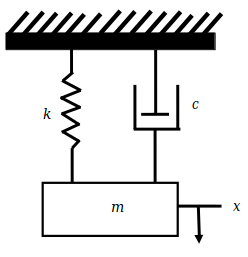
\includegraphics[width=5cm]{1.png}
  \caption{1自由度の振動系}
\end{figure}  
\\式(2)は,減衰自由振動を示し,時間とともに減衰していく性質を持っている.

\subsection{強制振動}
図1の振動系に$P_0\sin{\omega}{t}$の励振力が作用している場合の
運動方程式は,次式で表される.
\begin{equation}
  m\ddot{x}+c\dot{x}+kx = P_0\sin{\omega}{t}
\end{equation}
式(3)の解は時間が十分経過しているとすると,
\begin{equation}
  x = {\dfrac{p_0/m\omega_n^2}{\sqrt{(1-\gamma^2)^2+(2\zeta\gamma)^2}}\sin(\omega{t}-\theta)}
\end{equation}
のように近似できる.ここで,\\
\quad $\gamma=\omega/\omega_n$,$P_0$:励振力の振幅,
$\theta=\tan^{-1}{\dfrac{2\zeta\gamma}{1-\gamma^2}}$
:位相\\
である.式(4)は,時間が経過しても減衰することなく,定期的に持続する振動である.
このような励振力と同じ振動数を持った定常振動を強制振動という.

\subsection{実験装置}
\subsubsection{磁気ダンパの原理}
図2に磁気ダンパの正面断面図を,図3に側面図を示す. 
鉄心の両側には線径1mmの鋼線が200ターン巻かれており,
コイルに励磁電流を与えて磁束を発生させる. 
鉄心には, 空気層(以下ギャップと呼ぶ)が設けられており
銅版が挿入されている. ギャップ部に磁束を発生させた状態で
銅版が運動すると,フレミングの右手則に従って,
銅版に渦電流が発生する.この渦電流とギャップ部の磁束により,
フレミングの左手則に従って,電磁力が発生する.
この電磁力は銅版の運動と反対方向に生じるため,
振動を減衰させるダンパとして使用できる.

\begin{figure}[h]
  \begin{minipage}{0.5\hsize}
   \begin{center}
    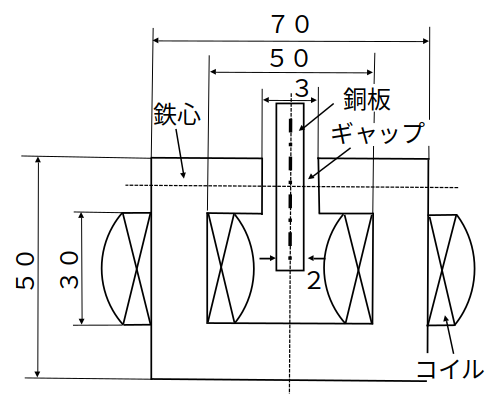
\includegraphics[width=5cm]{2.png}
   \end{center}
   \caption{磁気ダンパ正面断面図}
   \label{fig:one}
  \end{minipage}
  \begin{minipage}{0.5\hsize}
   \begin{center}
    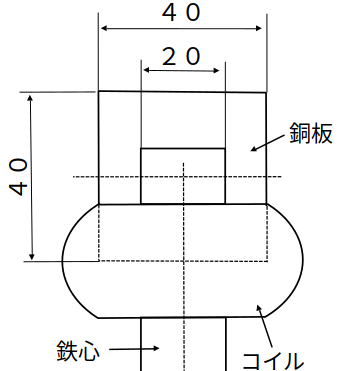
\includegraphics[width=5cm]{3.png}
   \end{center}
   \caption{磁気ダンパ側面}
   \label{fig:two}
  \end{minipage}
\end{figure}  

\subsubsection{実験システム構成}
図4に実験システムの概要を示す. 
アルミ版の片持ばりの先端付近に,磁気ダンパを設置して,
振動を減衰させる.磁気ダンパのコイルには,
DC電源から励磁電流を与えて磁束を発生させ,
減衰力を生じさせる. はり先端の下側には,
励振力を与えるために,加振器が設置してある.
加振増幅器から加振器に電圧を与えることにより,励振力を発.させる.
振動を計測するために,加速度センサーをはりに取り付けている. 
加速度センサーは,アンプで増幅した後,AD変換ボードを介してコンピュータに
取り込まれる.
\newpage

\begin{figure}[h]
  \centering
  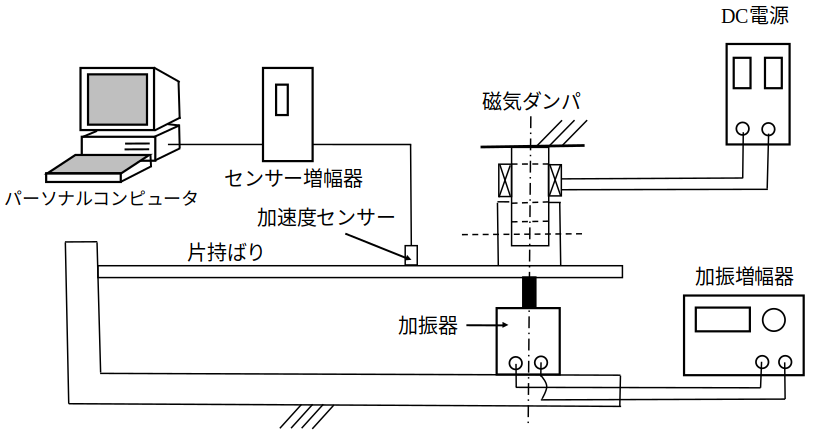
\includegraphics[width=10cm]{4.png}
  \caption{実験システムの概要}
\end{figure}


\subsubsection{使用器具}
\begin{itemize}
  \item DC電源  1台  菊水電子  MOEL PAD 35-5L
  \item 加速度センサー  1ケ  共和電業  AS-2GA YN5780
  \item 加振器  1台  IMV CORPORATION  MODEL PET-01
  \item 加振増幅器  1台  IMV CORPORATION  MODEL PET-0A
  \item AD変換モジュール  1枚  CONTEC  AD12-8(USB)GY
  \item パーソナルコンピューター  1式
\end{itemize}

\section{実験方法}
\subsection{減衰自由振動と強制振動の自動計測}
\subsubsection{実験準備}
\begin{enumerate}
  \item DC電源の出力端子と磁気ダンパのコイル端をリード線で接続する.
  \item センサー増幅器の出力をAD変換モジュールの0チャネルに接続する.
  \item 加振増幅器の出力端子と加振器の入力端子を接続する
  \item センサー増幅器の電源を入れる.
  \begin{itemize}
    \item パネル正面の電圧計のはりが0になっていないときは,
    その右側のBALつまみにより,零調整を行なう.
    \item $μ\epsilon$の値が615になっていることを確認する.
    \item パネル正面のCALつまみを上にたおし,
    電圧が+5[V]になることを確認する.+5[V]にならないときは,
    VERNつまみを調整して+5[V]に設定する.
    これで1G(9.8[m/s2])が5[V]になるように校正できる.
  \end{itemize}
  \item パソコンの電源を入れ,コマンドプロンプトを立ち上げる.
\end{enumerate}

\subsubsection{減衰自由振動の計測}
\begin{enumerate}
  \item 励磁電流を0[A] から3[A] の4通りについて計測を行う,
  励磁電流を0[A] にして計測するときには, DC電源をOFFにする.
  \item 励磁電流の設定が終れば,キーボードから 『ad dampO.dat  $\hookleftarrow$』 と入力する.
  ただし, damp0.dat は励磁電流を 0[A] に設定し計測するデータファイルである.
  \item 指で,はりに2-3[mm] 程度の初期変位を与え, 指を離た直後に$\hookleftarrow$を押し, 
  自由振動の計測を行う.
  \begin{itemize}
    \item AD変換が始まり, 加速度に比例した電圧値が, コンピュータに取り込まれる. $1G(9.8[m/s^2])$ 
    が5[V] になるように設定しているので,取り込まれた電圧値は,加速度に変換され, 
    指定したデータファイル名のデータファイルに書き込まれる.
  \end{itemize}
  \item 励磁電流を1, 2, 3 [A] に設定して同様に計測する.
  データファイル名 (damp$i$.dat) は,設定した磁電流$i$[A] である. 
\end{enumerate}

\subsubsection{強制振動の計測}
\begin{enumerate}
  \item DC電源のVOLTAGEのつまみを調節して電流を1[A]に設定する.
  \item 加振増幅器の正面パネル左下方にある電源スイッチをONにする.
  \begin{itemize}
    \item 加振増幅器の正面パネル左下方, SELECTOR(Hz)のボタンのうち2-20[Hz]のボタンを押して,
    周波数範囲を設定する. GATE は OFF にする.
    \item 中央付近, ATT は 20 [dB] にする.OUTPUT つまみは,白線がほぼ真上にくるように設定する.
    \item FREQUENCY のつまみを左側いっぱいに回す.このとき助振力の周波数は[2Hz] となる.
  \end{itemize}
  \item FREQUENCY のつまみをゆっくり時計回りに回し,周波数を2[Hz] から 20[Hz]まで,
  ゆっくりと変化させる. 
  周波数が10[Hz]付近でが大きくなり,10[Hz]から離れるにつれて動が小さくなることを観測する. このように,力のある周波数で,振動が大きくなる現象を共という.
  \item 加振増幅器の周波数を10 [Hz] に設定する. 次に, GATE を ON にして 10.0 [Hz] に微調整する GATE を ONにしたときは,
  周波数が表示されるまで, 10 秒を必要とするので注意する. 
  \item キーボードから『adf vib1.dat  $\hookleftarrow$』 と入力する. 
  ただし, vib1.dat は励磁電流を1[A] に設定し計測するデータファイルである.
  \begin{itemize}
    \item  AD変換が始まり, 加速度センサーの電圧信号は,AD変換されてコンピュータに取り込まれる.
    このデータは,校正値により加速度に変換され,指定したデータファイル名のデータファイルに書き込まれる.
  \end{itemize}
  \item 周波数はそのままで,励磁電流を2,3,4[A] に設定し,同様の実験を行なう. 励磁電流 $i$[A] における共振時の強制振動波形を vibidat に書き込む.
  
  (注意) 励磁電流を長時間与え続けると, ダンパのコイル部が加熱するので,できるだけすみやかに実験を行なうこと.
\end{enumerate}

\subsubsection{グラフの作成}
\begin{enumerate}
  \item 減衰自由振動の計測
  \begin{itemize}
    \item 磁気ダンパの励磁電流が 0,1,2,3 [A] における減衰自由振動波形を描き,考察して報告する.
  \end{itemize}
  \item 強制振動の計測
  \begin{itemize}
    \item 励振力の周波数 10.0 [Hz], 励磁電流が 1,2,3,4 [A] における強制振動波形を描き, 考察して報告する.
  \end{itemize}
\end{enumerate}

\subsection{データの処理}
WebClass から gensui.xsl, dft.xsl をデータファイルと同じ場所にコピーする.

\subsubsection{グラフの作成}
\begin{enumerate}
  \item データファイルに書き込まれた加速度の減衰自由振動波形を読み込み,平均化, ピーク値および複振幅の抽出,
  復振幅の正規化の処理を行なう. これらの値から最小二乗法を用いて減衰比を計算する.
  \begin{itemize}
    \item 縦軸に番目の復振幅 $W_i(i=1,...,n-1)$, 
    横軸に $i+1$番目の復振幅 $W_i+1 (i=1,...,n-1)$ をとれば,ほぼ直線のグラフが得られる. 
    このグラフを描くために, Excel のマクロを用い各復振幅の値を正規化し,シートに書き込む,
    また, 計算過程, 減衰比の値を記録するために 別のシートに保存する.
  \end{itemize}
  \item 配布した gensui.xls を Excel で開き,マクロを有効にする.『表示』→『マクロ』から『Open Dat』を実行し,処理を開始する.
  このとき, damp$i$.dat$(i=0,...,3)$ から減衰自由振動波形のデータを読み込み, 
  処理を行ない,減衰比などの 計算結果をシート 『GENSUI』 に, 
  グラフ作成用のデータを測定結果と共にシート『DAMP$i$ $(i=0,...,3)$』に 書き込む.
  (注意) 減衰自由振動の測定結果のデータファイル名は,damp$i$.dat$(i=0,...,3)$ でなければなく,ファイル名が異なる場合は名前を変更する.
  \item シート『DAMP$i (i=0,...,3)$』の「解析データ」のグラフを描けば, 横軸を$i+1$番目の複振幅 $W_i+1$,
  縦軸を$i$番目の復振幅$W_i$, とした, ほぼ直線のグラフが得られる.励磁電流値が0,1,2,3[A]におけるグラフを同時に描き, 比較考察する.
  \item 励磁電流値 (Exciting current) $i$ を横軸に,
  減衰比 $\zeta$ (Damping ratio) を縦軸にとり, グラフに整理して考察する(表も作成).
\end{enumerate}

\subsubsection{DTF(デジタル信号の周波数解析)}
\begin{enumerate}
  \item 強制振動波形のデータを読み込み, 平均化, DFT の信号処理を行なう. 
  スペクトルの周波数応答をグラフ表示するため,シートに DFT 結果を書き込むとともに,
  卓越ピーク値とその周波数を別のシートに保存する.
  \item 配布した dft.xls を Excel で開き, マクロを有効にする.
  『表示』→『マクロ』から『OpenDat』を実行し,処理を開始する.
  このとき, vib$i$.dat $(i=1,..., 4)$ から強制振動波形のデータを読み込み, 
  処理を行ない, 卓越ピーク値などの計算結果をシート 『DFT』 に,グラフ作成用データを測定結果と共にシート 
  『VIB$i(i=1,...,4)$』に書き込む. \\
  (注意) 強制振動の測定結果のデータファイル名は,
  vib$i$.dat$(i=1,..., 4)$ でなければなく, ファイル名が異なる場合は名前を変更する.
  \item シート 『VIB$i(i=1,..., 4)$』 の「解析データ」をグラフ表示する. 
  横軸は周波数 $Hz$, 縦軸は振動加速度のスペクトル$m/s^2$ になっている. 横軸,縦軸ともに対数スケールにして表示する.
  \item 励磁電流の変化に対する卓越ピーク値 (スペクトルの最大値)をグラフ表示し,
  共振の抑制効果について考察する. 横軸に励磁電流値 A, 縦軸に加速度の卓越ピーク値$m/s^2$ をとりグラフを描く (表も作成).
\end{enumerate}
\section{実験結果}
\subsection{減衰自由振動の計測結果}
図5から図8に減衰自由振動波形を,図9に復振幅の比のグラフを,図10に励磁電流と減衰比の関係性を示すグラフと表を示す.
\newpage
\begin{figure}[h]
  \centering
  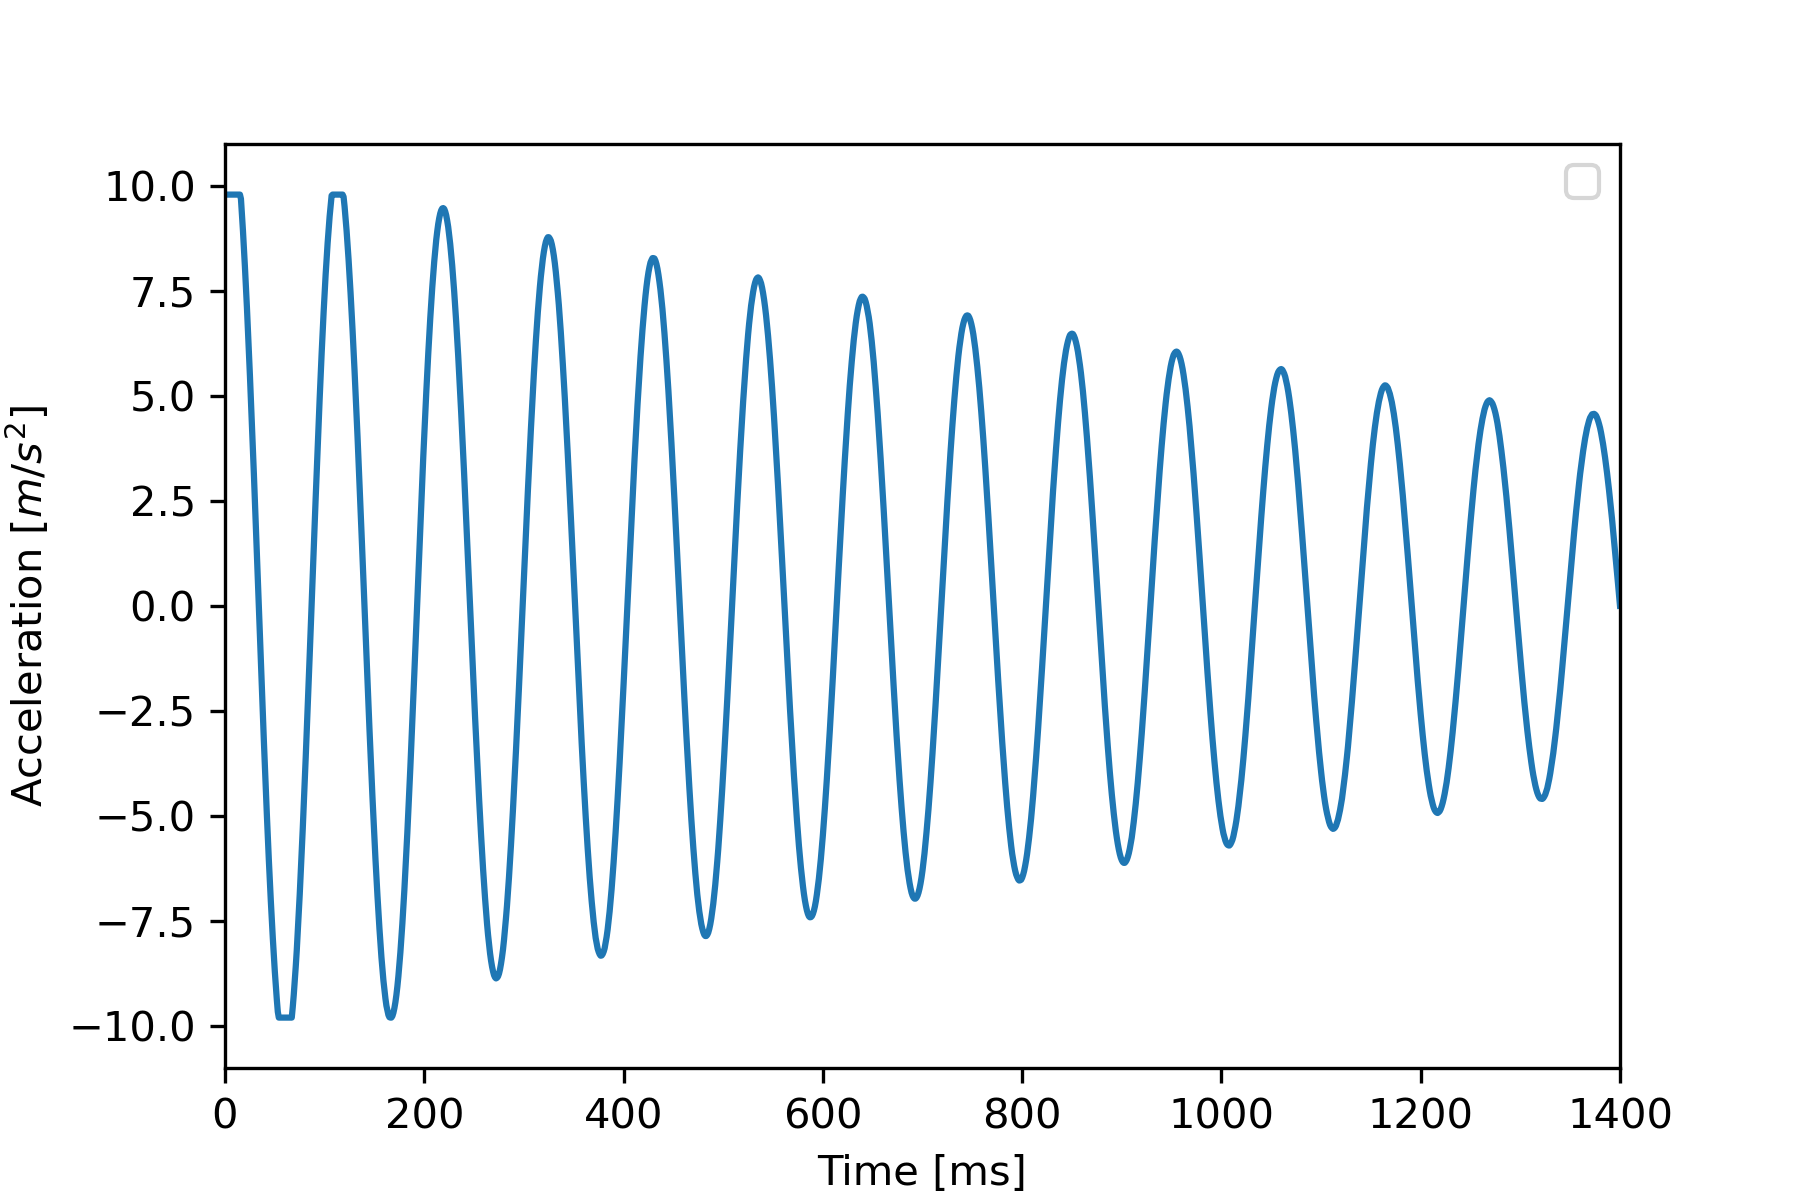
\includegraphics[width=13cm]{damp0.png}
  \caption{励磁電流が0[A]のときの減衰自由振動波形}
\end{figure}
\begin{figure}[h]
  \centering
  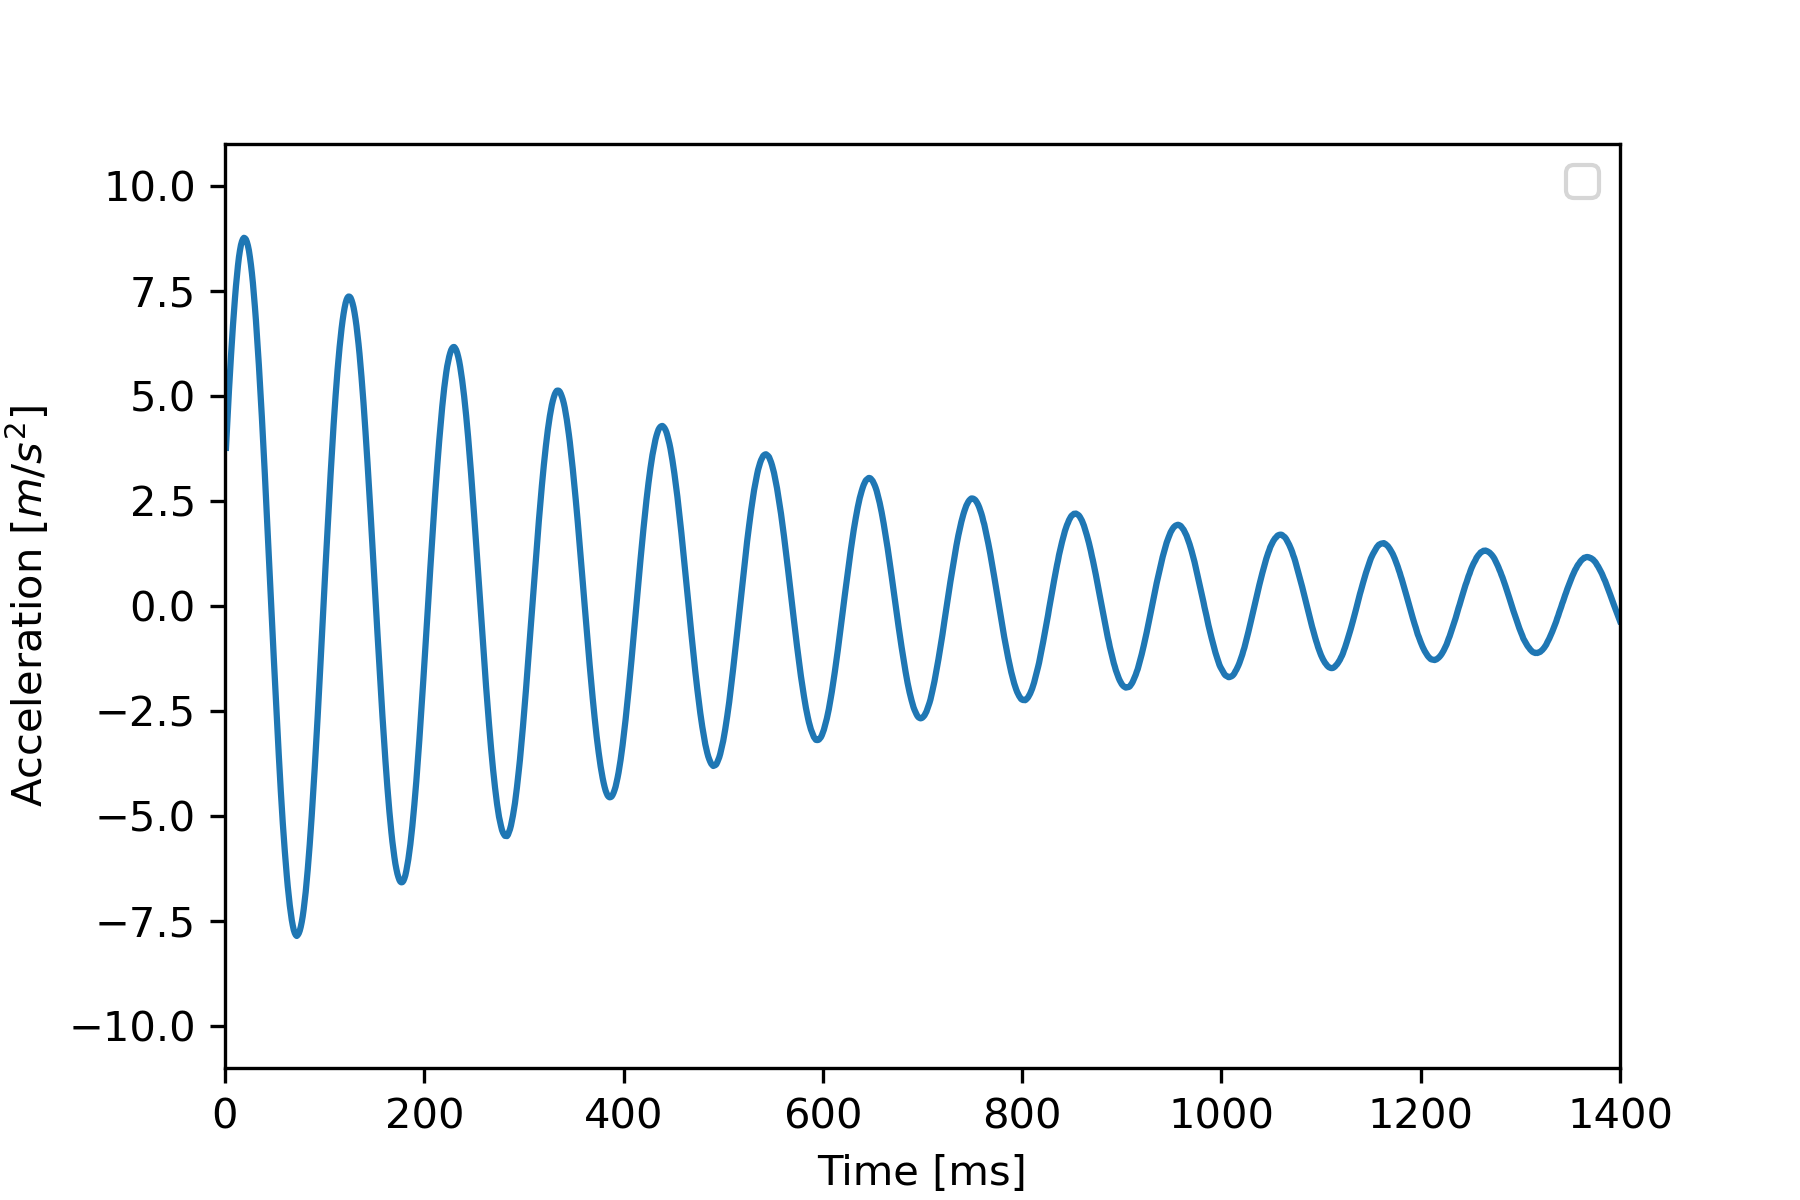
\includegraphics[width=13cm]{damp1.png}
  \caption{励磁電流が1[A]のときの減衰自由振動波形}
\end{figure}
\newpage
\begin{figure}[h]
  \centering
  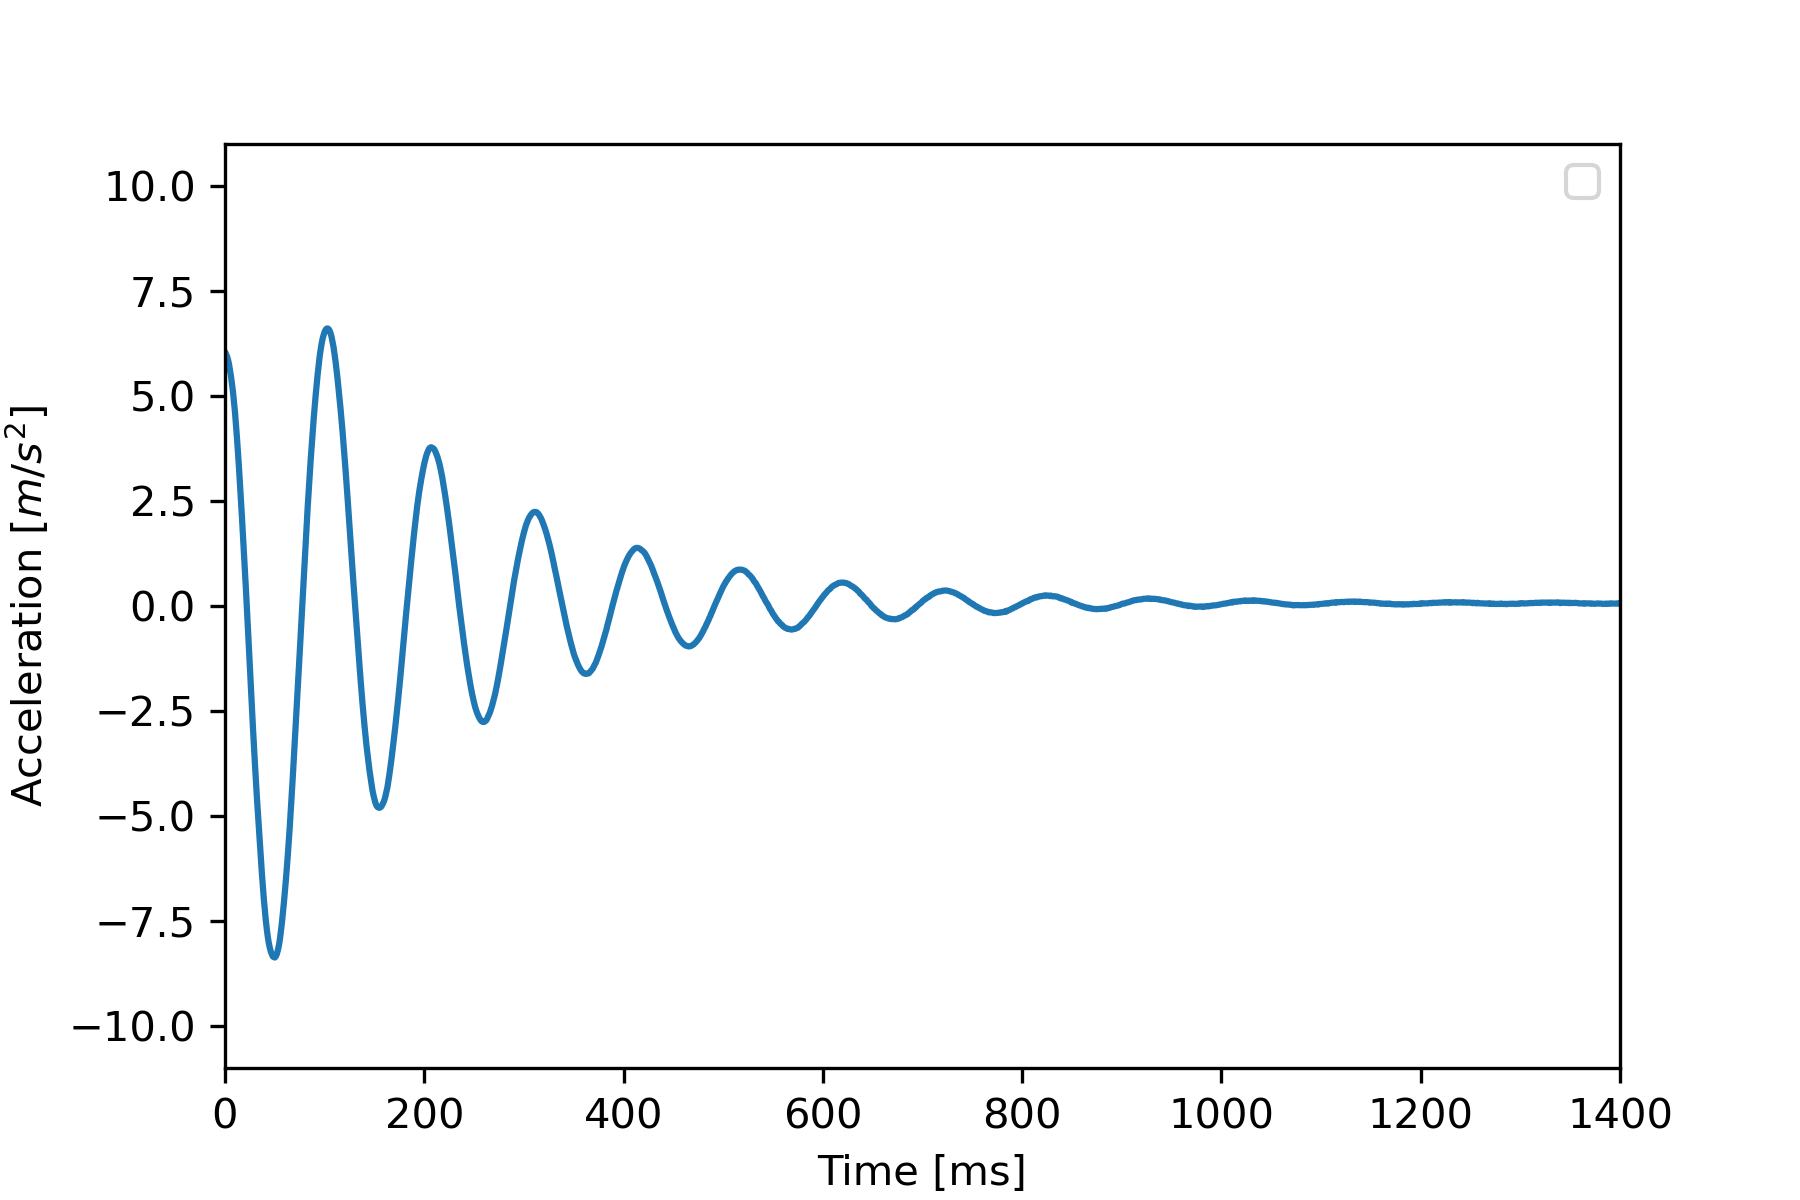
\includegraphics[width=13cm]{damp2.png}
  \caption{励磁電流が2[A]のときの減衰自由振動波形}
\end{figure}
\begin{figure}[h]
  \centering
  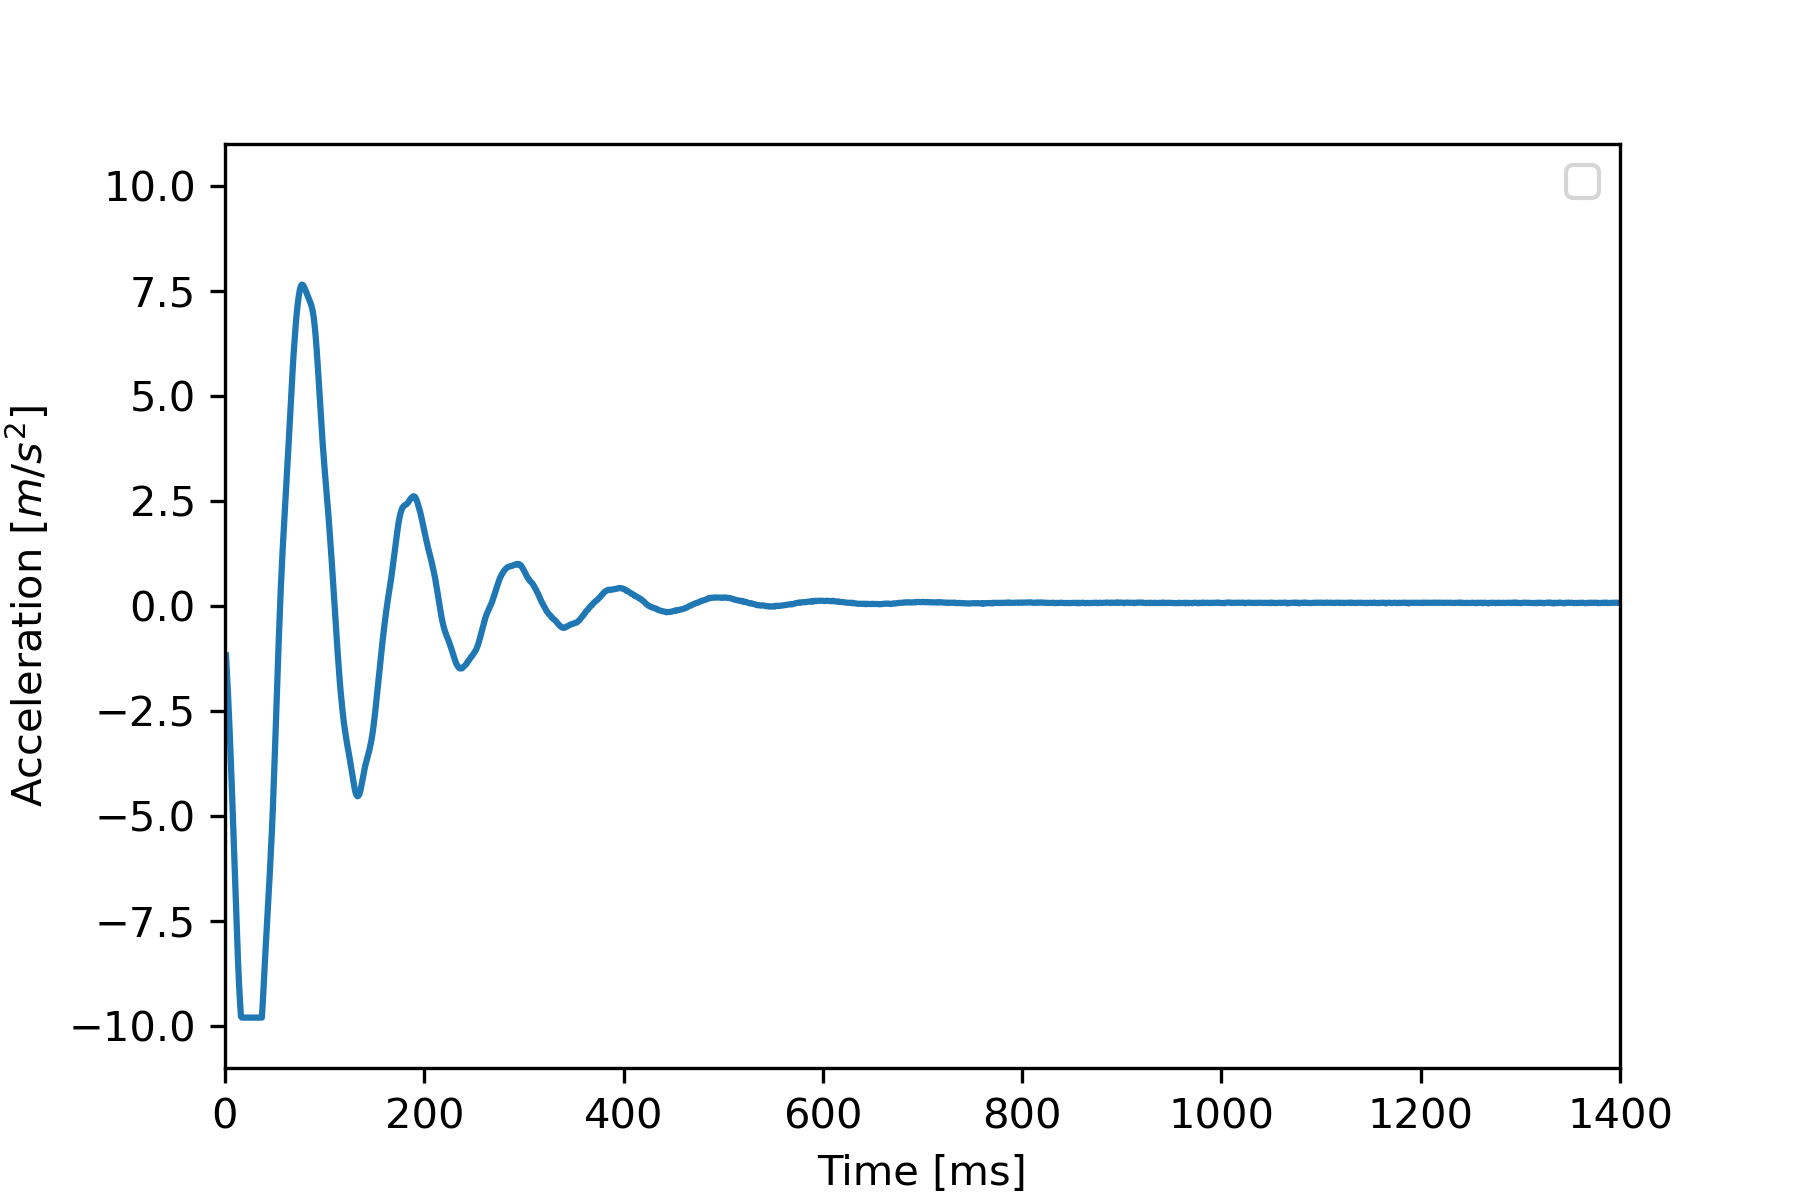
\includegraphics[width=13cm]{damp3.png}
  \caption{励磁電流が3[A]のときの減衰自由振動波形}
\end{figure}
\newpage
\begin{figure}[h]
  \centering
  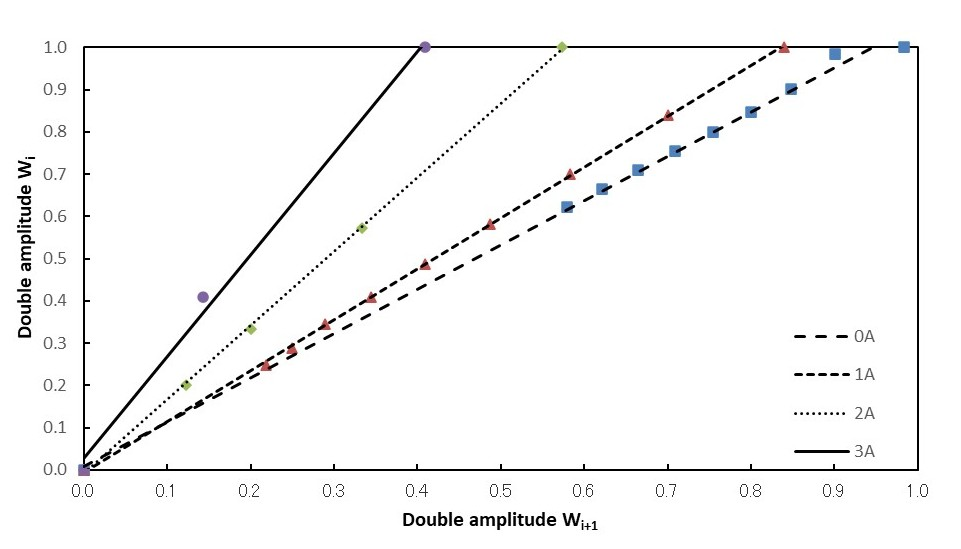
\includegraphics[width=13cm]{5.png}
  \caption{各励磁電流での復振幅の比}
\end{figure}
\begin{figure}[h]
  \centering
  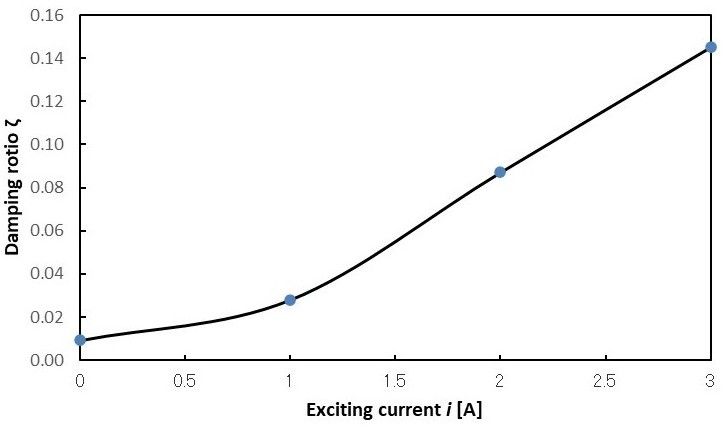
\includegraphics[width=13cm]{6.png}
  \caption{励磁電流と減衰比の関係比}
\end{figure}
\newpage
\begin{table}[h]
  \centering
  \caption{励磁電流と減衰比の関係}
  \begin{tabular}{l|c|r}
    励磁電流[A]&減衰比\\\hline\hline
      0&0.009249 \\ \hline
      1&0.028072  \\
      2&0.087142  \\
      3&0.145136  \\\hline
  \end{tabular}
\end{table}


\subsection{強制振動の計測結果}
図11から図14に強制振動波形を,図15から図18に周波数と振動加速度のスペクトルのグラフを,図19と表2に励磁電流と卓越ピーク値のグラフと表を示す.

\begin{figure}[h]
  \centering
  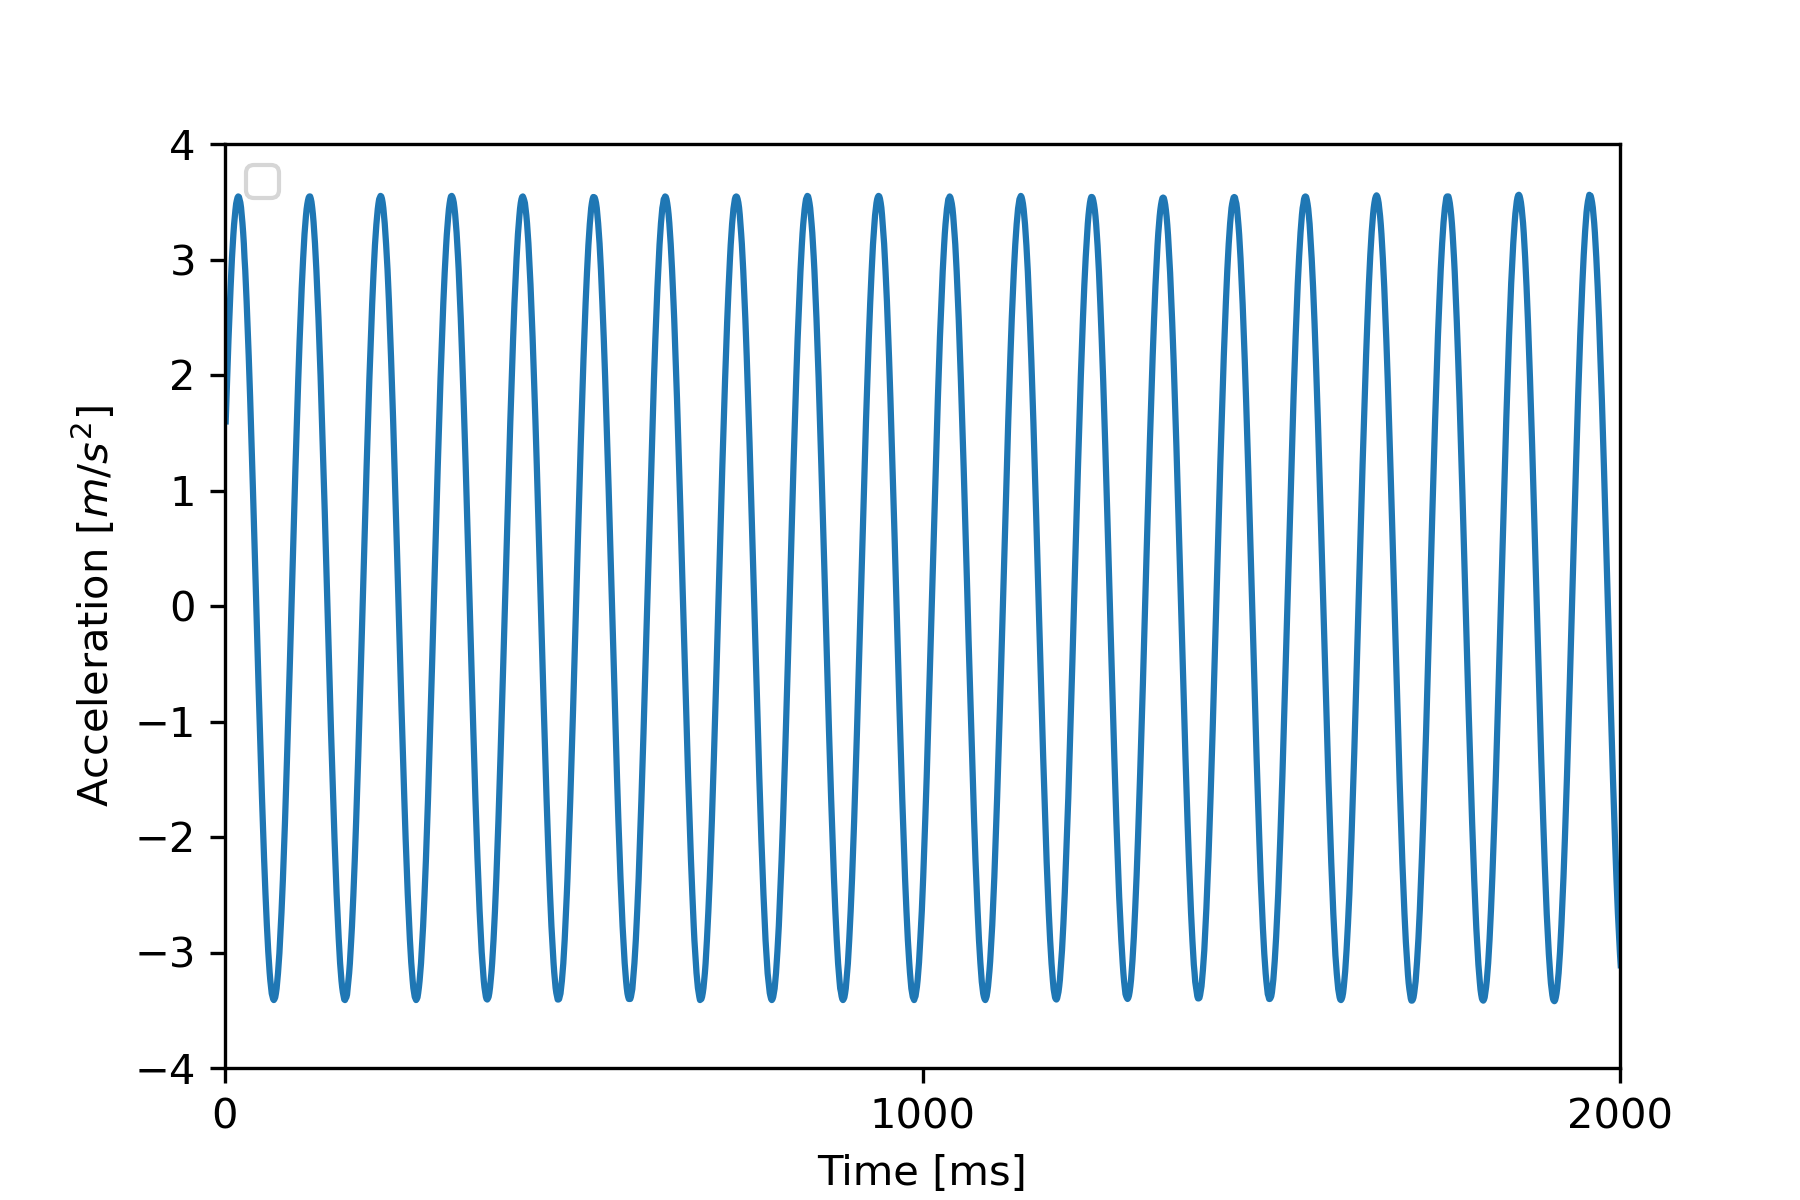
\includegraphics[width=14cm]{vib1.png}
  \caption{励磁電流が0[A]のときの強制振動波形}
\end{figure}
\begin{figure}[h]
  \centering
  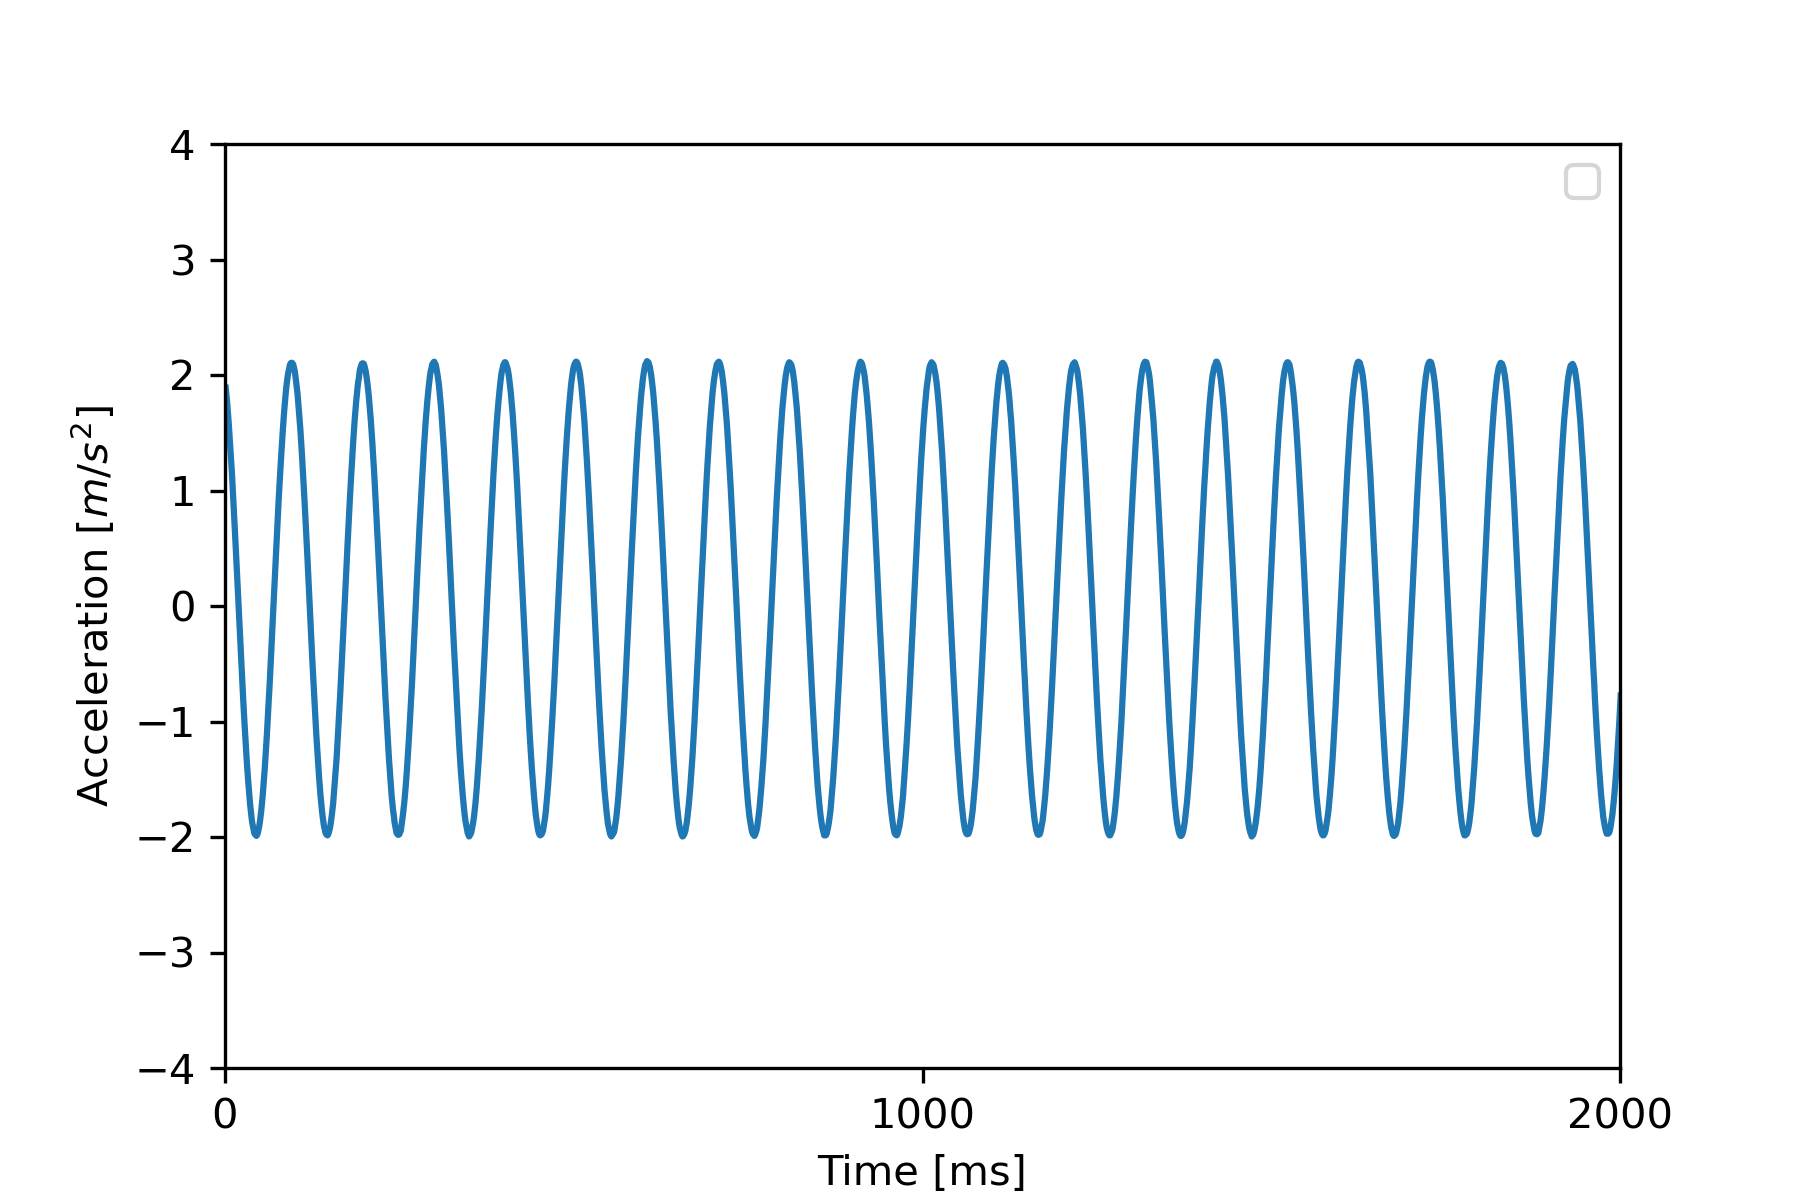
\includegraphics[width=14cm]{vib2.png}
  \caption{励磁電流が1[A]のときの強制振動波形}
\end{figure}
\newpage
\begin{figure}[h]
  \centering
  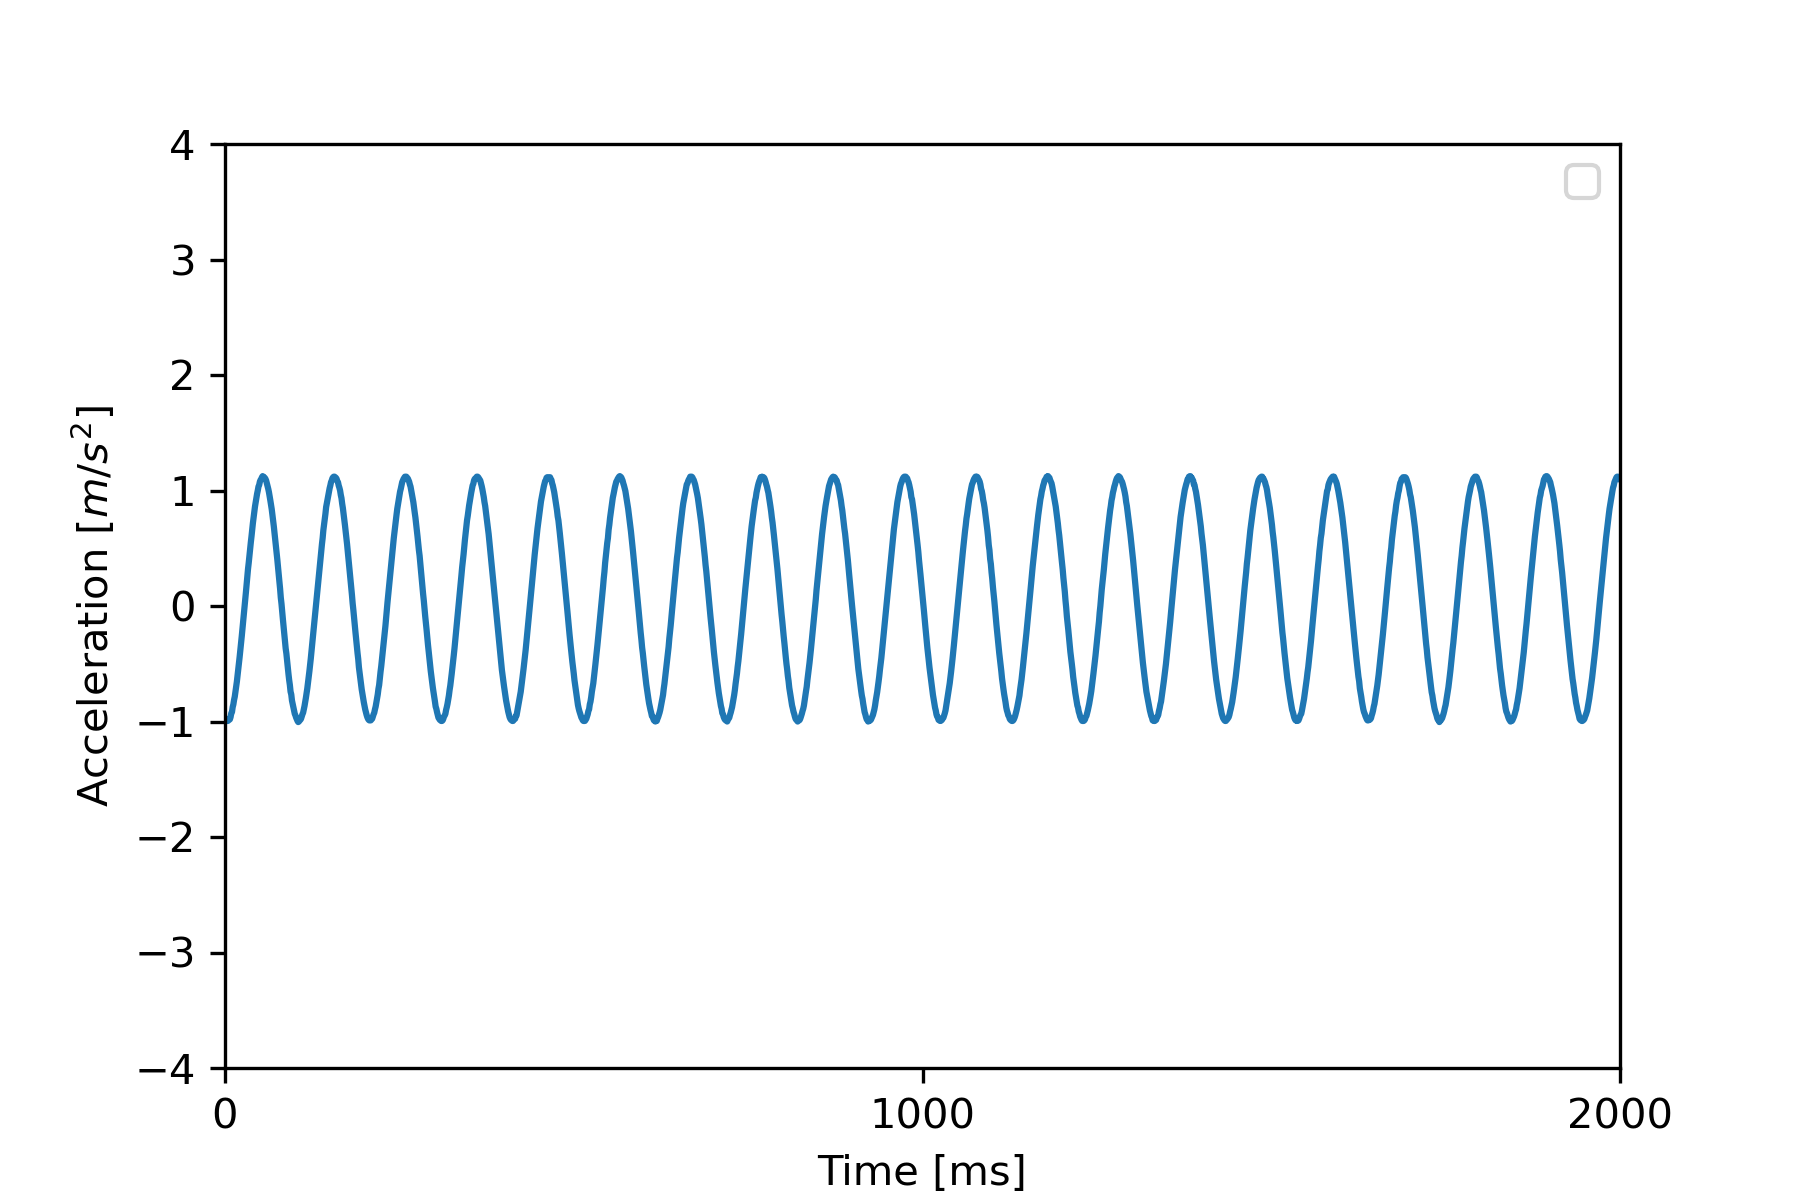
\includegraphics[width=14cm]{vib3.png}
  \caption{励磁電流が2[A]のときの強制振動波形}
\end{figure}
\begin{figure}[h]
  \centering
  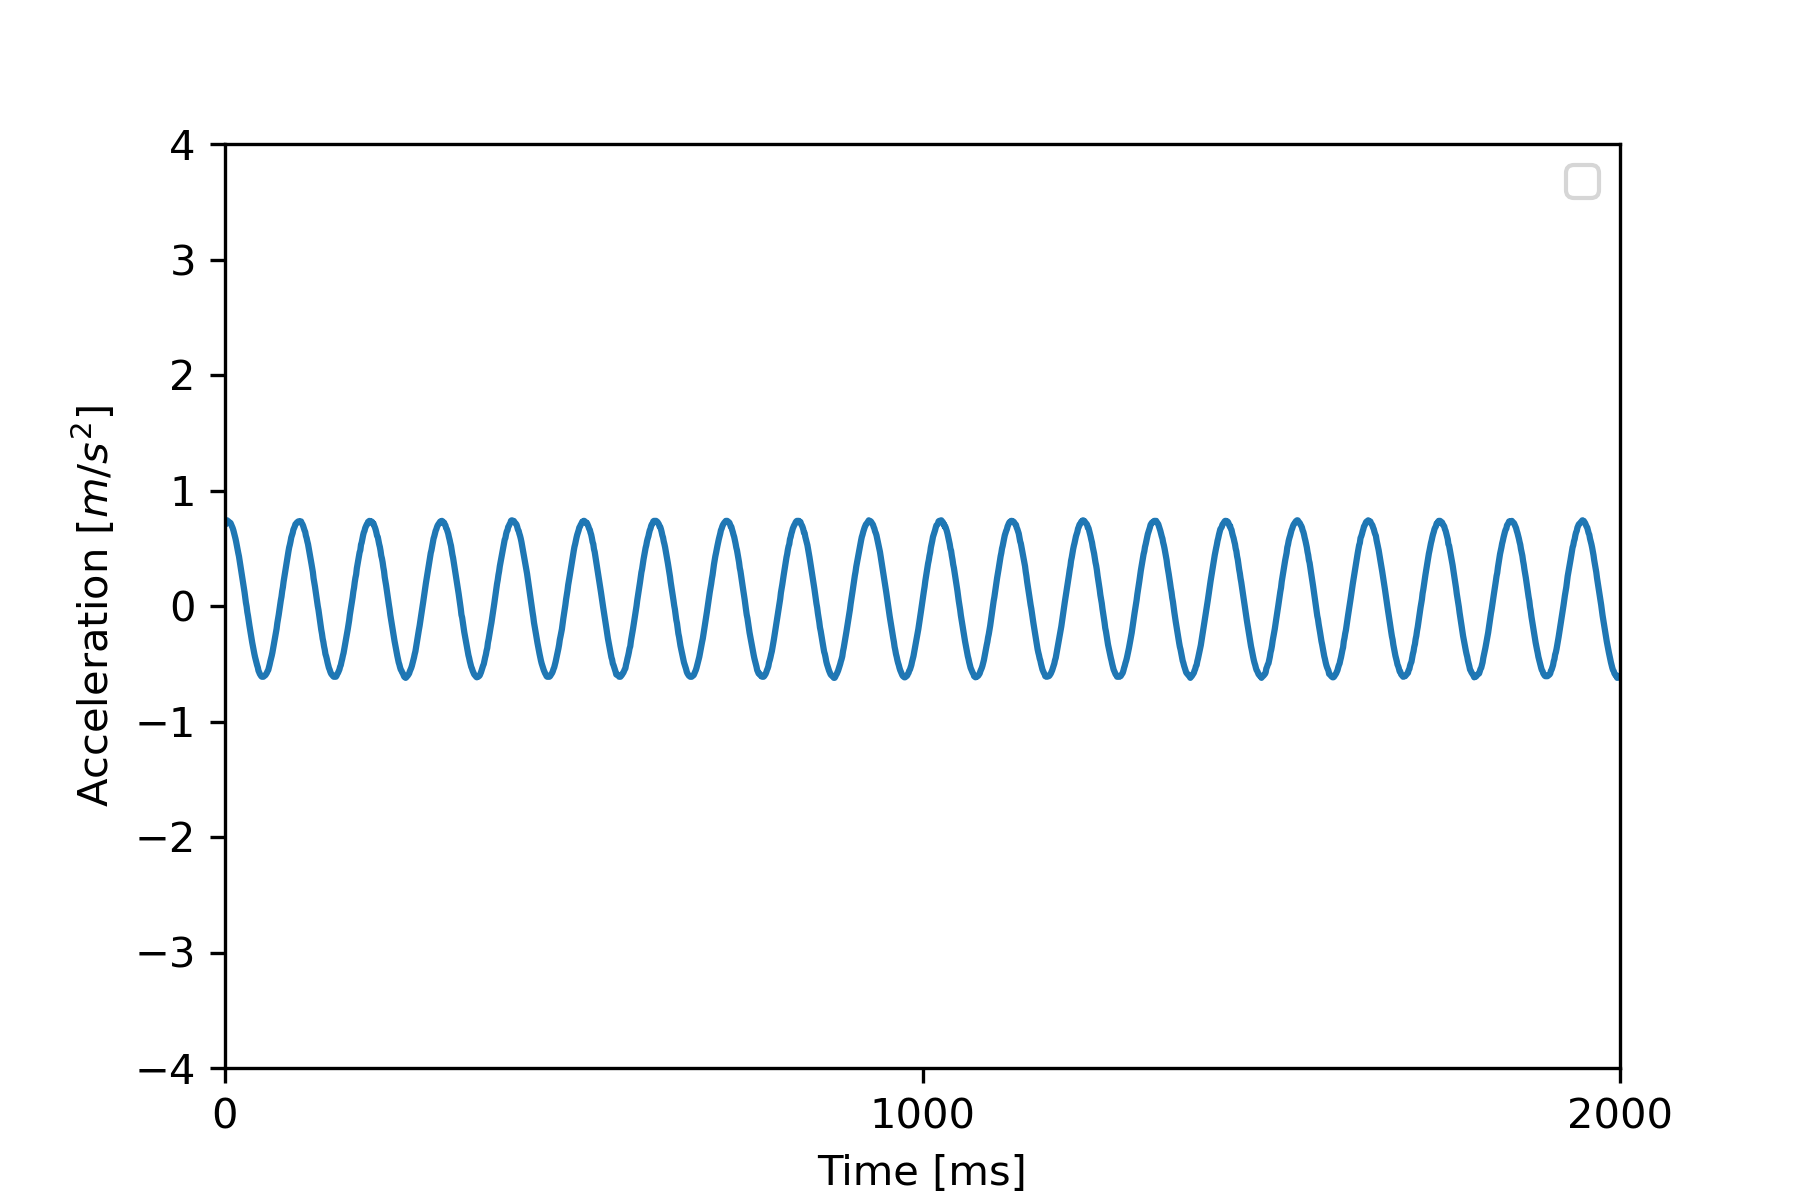
\includegraphics[width=14cm]{vib4.png}
  \caption{励磁電流が3[A]のときの強制振動波形}
\end{figure}
\newpage
\begin{figure}[h]
  \centering
  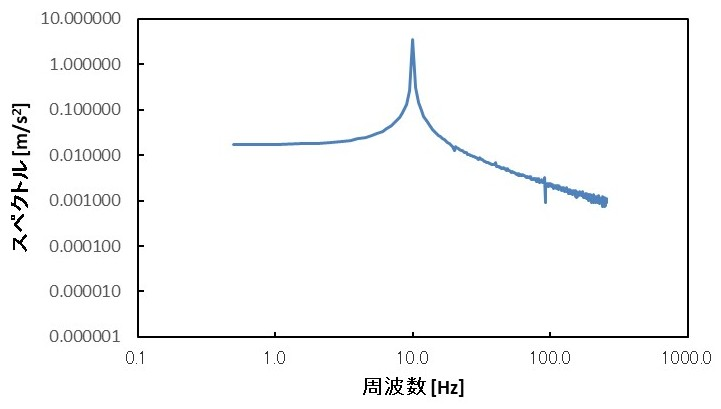
\includegraphics[width=14cm]{7.png}
  \caption{励磁電流が0[A]のときの周波数と振動加速度のスペクトル}
\end{figure}
\begin{figure}[h]
  \centering
  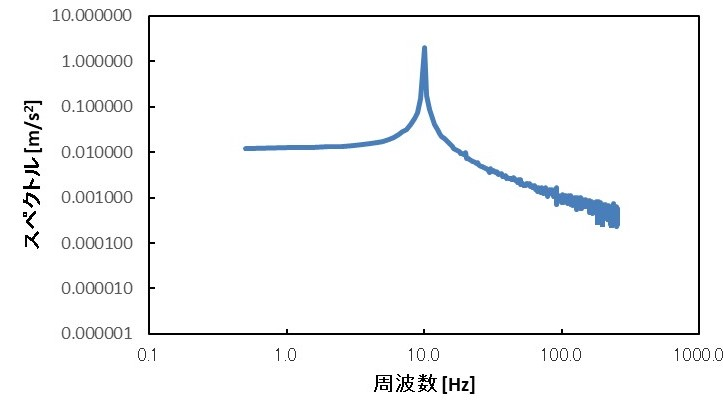
\includegraphics[width=14cm]{8.png}
  \caption{励磁電流が1[A]のときの周波数と振動加速度のスペクトル}
\end{figure}
\newpage
\begin{figure}[h]
  \centering
  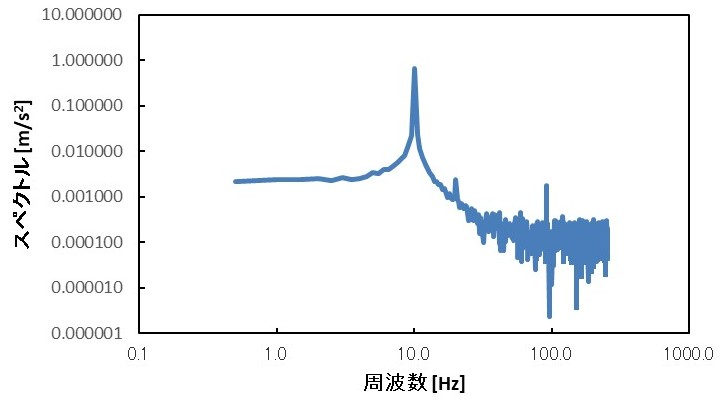
\includegraphics[width=14cm]{9.png}
  \caption{励磁電流が2[A]のときの周波数と振動加速度のスペクトル}
\end{figure}
\begin{figure}[h]
  \centering
  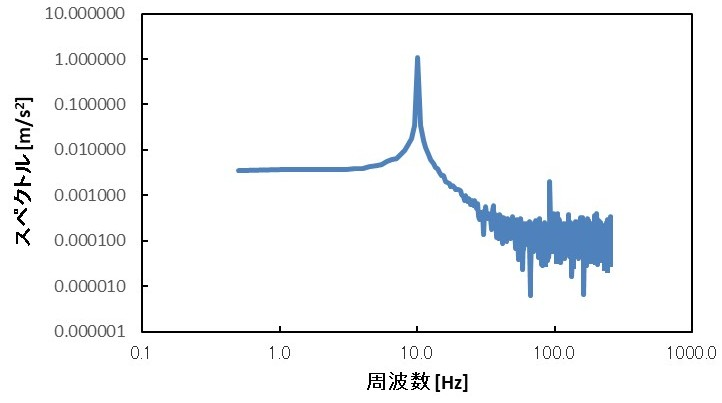
\includegraphics[width=14cm]{10.png}
  \caption{励磁電流が3[A]のときの周波数と振動加速度のスペクトル}
\end{figure}
\newpage

\begin{figure}[h]
  \centering
  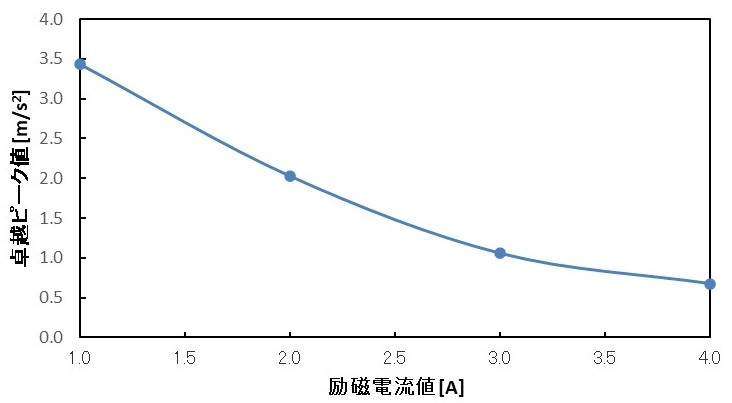
\includegraphics[width=14cm]{11.png}
  \caption{励磁電流と卓越ピーク値}
\end{figure}
\newpage
\begin{table}[h]
  \centering
  \caption{励磁電流と卓越ピーク値の関係}
  \begin{tabular}{l|c|r}
    励磁電流[A]&卓越ピーク値$[m/s^2]$\\\hline\hline
      1&3.435580 \\ \hline
      2&2.025797  \\
      3&1.056152  \\
      4&0.673936  \\\hline
  \end{tabular}
\end{table}

\section{考察}
\subsection{減衰自由振動}
\subsubsection{減衰自由振動の計測}
図5〜8よりすべて復振幅が0へ収束している.これは式(2)より$t$が大きくなる,つまり時間が経てば運動が減衰していることを
表しているためである.
また,励磁電流が大きくなるほど,
減衰自由振動波形の大きさが小さくなっているのがわかる.これは励磁電流を高めることにより,磁力が大きくなり
減衰力が強くなるためだと考えられる.
\subsubsection{減衰比の計算}
図9の各励磁電流での復振幅の比のグラフと図10励磁電流と減衰比の結果より,励磁電流が大きくなると
減衰比が大きくなっており,考察6.1.1と同じく励磁電流を高めることにより,磁力が大きくなり
減衰力が強くなるためだと考えられる.
では図1について考える.
式(1)より
\begin{equation}
  \ddot{x}+2\zeta\omega_n\dot{x}+\omega_n^2x = 0
\end{equation}
となる.これは減衰のある1自由度振動系の標準形である.
$\omega_n$は固有角振動数であり固有振動の振幅は初期値には依存するが,固有角振動数は系の固有の値であって,
期待値に関係ない.式(5)は提携数の線形状微分方程式であるが$\sin\omega_{n}t$や$\cos\omega_{n}t$などは解ではない.
そこで解として$x=Ae^{st}$とし解を求める.
\begin{equation}
  A(S^2+2\zeta\omega_{n}s+\omega^2)e^{st} = 0
\end{equation}
$e^{st}$は零ではないから,上の式がA=0以外の解をもつためにはsが
\begin{equation}
  S^2+2\zeta\omega_{n}s+\omega^2= 0
\end{equation}
という代数方程式の根であればよい.これを式(5) の特性方程式という.
式(6)の2根を$s_1,s_2$とする.
\begin{equation}
  s_1,s_2= (-\zeta\pm\sqrt{\zeta^2-1})
\end{equation}
よって$\zeta>1$では実数の相異なる2根をもち,$\zeta=1$では重根,$\zeta<1$では虚根を持つ.
減衰係数$c$が小さければ$\zeta$は小さくなる.次に方程式の解を小さい順に示す.\\
$\zeta<1$場合
\begin{equation}
  x=ae^{-\zeta\omega_{n}t}\cos(qt-\phi)
\end{equation}
$\zeta=1$場合
\begin{equation}
  x=(x_o+(v_0+1\omega_nx_0)t)e^{-1\omega_nt}
\end{equation}
$\zeta>1$場合
\begin{equation}
  x=e^{-\zeta\omega_{n}t}(x_o\cos{h}q't+\dfrac{v_0+\zeta\omega_nx_0}{q'}\sin{hq't})
\end{equation}
となる.

\subsection{強制振動}
\subsubsection{強制振動の計測}
図11〜14より強制振動波形が常に一定の振動をしていることがわかる.
また,励磁電流が大きくなればなるほど振動の大きさが小さくなっている.これも励磁電流を高めることにより,磁力が大きくなり
減衰力が強くなるためだと考えられる.
\subsubsection{DFT(デジタル信号の周波数解析)}
図15〜18より,どの励磁電流でも10[Hz]のときが一番スペクトルが大きくなっている.また励磁電流が大きくなればなるほど
スペクトルが小さくなっている.また図19より励磁電流が大きくなればなるほど卓越ピーク値が下がっており,共振が抑制されている
ことがわかる.
\section{課題}
\begin{enumerate}
  \item 
対数減衰率$\delta$は,減衰自由振動の隣り合う振幅の比の自然対数のことである.そのため次式のようになる.
\begin{equation}
  \delta = {ln\dfrac{W_i}{W_{i+1}}}
\end{equation}
式(2)より
\begin{equation}
  W_i = {\dfrac{x_0}{\sqrt{1-\zeta^2}}e^{-\zeta {\omega}_{n} t_i}\cos (qt_i-\phi)}
\end{equation}
\begin{equation}
  W_{i+1} = {\dfrac{x_0}{\sqrt{1-\zeta^2}}e^{-\zeta {\omega}_{n} t_{i+1}}\cos (qt_{i+1}-\phi)}
\end{equation}
とわかるので対数減衰率$\delta$は
\begin{equation}
  \delta = ln{\dfrac{\dfrac{x_0}{\sqrt{1-\zeta^2}}e^{-\zeta {\omega}_{n} t_i}\cos (qt_i-\phi)}{\dfrac{x_0}{\sqrt{1-\zeta^2}}e^{-\zeta {\omega}_{n} t_{i+1}}\cos (qt_{i+1}-\phi)}}
\end{equation}
となる.
なお式(6)(7)のとき$(qt_{i}-\phi)$が$2i\pi$であるときが振幅が一番大きくなるため,
\begin{equation}
  t_i = {\dfrac{2i\pi+\phi}{q}}
\end{equation}
\begin{equation}
  t_{i+1} = {\dfrac{2(i+1)\pi+\phi}{q}}
\end{equation}
となる.
このとき$(t_{i+1}-t_{i})$は
\begin{equation}
  t_{i+1}-t_{i} = {\dfrac{(2(i+1)\pi+\phi)-2i\pi+\phi}{q}} = {\dfrac{2\pi}{q}}
\end{equation}
となる.次に極大値の比は
\begin{equation}
  {\dfrac{W_i}{W_{i+1}}} = e^{{2\pi\zeta\omega_n}/q} = e^{\dfrac{2\pi\zeta}{\sqrt{1-\zeta^2}}}
\end{equation}
となる.よって1サイクルにおける減衰比の自然対数は
\begin{equation}
  \delta = log_e{e^{\dfrac{2\pi\zeta}{\sqrt{1-\zeta^2}}}} = {\dfrac{2\pi\zeta}{\sqrt{1-\zeta^2}}}
\end{equation}
となる.図9の傾きは$\delta$大きさを表している.
  \item $\delta$が小さい場合,
  \begin{equation}
    \delta = {\dfrac{2\pi\zeta}{{1}}}
  \end{equation}
  より,
  \begin{equation}
    \zeta = {\dfrac{\delta}{{2\pi}}}
  \end{equation}
  となる・

  \item 共振は,外力の周波数が共振系の固有振動数と一致するときに生じる.式(4)
    $x = \frac{{p_0/m\omega_n^2}}{{\sqrt{{(1-\gamma^2)^2+(2\zeta\gamma)^2}}}}\sin(\omega{t}-\theta)$
  において,分母の項が減衰比$\zeta$ に関連している.
  減衰比$\zeta$ の値が大きいほど,分母の値が大きくなり,共振の効果を抑えることができる.
  次を積分すると
  \begin{equation}
   {{(1-\gamma^2)^2+(2\zeta\gamma)^2}} 
  \end{equation}
  となり
  \begin{equation}
    -4\gamma(1-\gamma^2)^2+8\zeta^2\gamma
  \end{equation} 
  つまり$-4\gamma[(1-2\zeta^2)-\gamma^2]$なので$\gamma$が次のようである必要がある.
  \begin{equation}
   \gamma={\sqrt{1-2\zeta^2}}
  \end{equation}  
  これを式(23)に入れると
  \begin{equation}
    4\zeta^2(\zeta^2+(1-2\zeta^2))
  \end{equation}    
  となり$\zeta=0$とすると0となり分母が0となった.
  \begin{equation}
  x = \frac{{p_0/m\omega_n^2}}{{\sqrt{{4\zeta^2(\zeta^2+(1-2\zeta^2))}}}}\sin(\omega{t}-\theta)
    = \frac{{p_0/m\omega_n^2}}{{\sqrt{{0(0+(1-0))}}}}\sin(\omega{t}-\theta)
\end{equation} 
\\

  \item 
  フレミングの右手則(図21)は,導体が磁界中で運動するときに発生する起電力の向きを求めるときに使う.
  フレミングの左手則(図22)は,導体に電流が流れるときに受ける力の向きを求めるときに使う.
  応用例としては,右手則は発電機やダイナモなどの原理に使われる.
  左手則は電動モーターや電磁石などの原理に使われる. 
  \newpage
  \begin{figure}[h]
    \centering
    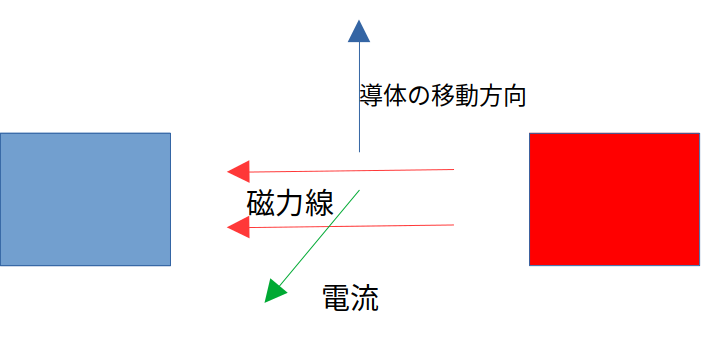
\includegraphics[width=10cm]{12.png}
    \caption{フレミングの右手則}
  \end{figure}
  \begin{figure}[h]
    \centering
    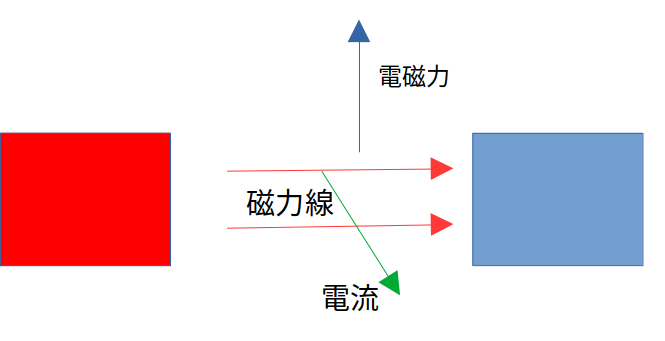
\includegraphics[width=10cm]{13.png}
    \caption{フレミングの左手則}
  \end{figure}
\end{enumerate}

\begin{thebibliography}{20}
  \bibitem{} 
  田村章義, 機械力学, 森北出版, 1990.
  \bibitem{}
  田中勝廣, 電磁気学, 日本理工出版会, 1987.
  \bibitem{}
  添田 喬, 得丸 英勝, 中溝 高好; 岩井 善太,振動工学の基礎 (増補改訂版)  , 日新出版 ,2013. 
 \end{thebibliography}

\end{document}
